\documentclass[8pt]{beamer}
\usepackage{tikz}
\usepackage[utf8]{vietnam}
\usepackage{amsmath}
\usepackage{graphicx}
\usepackage{wrapfig}
\usepackage{hyperref}
\usetheme{Copenhagen}
\usecolortheme{beaver}
\setbeamertemplate{navigation symbols}{}
\setbeamertemplate{headline}{}
\title[Chương 2: Hệ thống LTI] %optional
{Chương 2: Hệ thống LTI}
\subtitle{Tín hiệu và hệ thống}
\author[Tín hiệu và hệ thống] % (optional)
{Tín Vũ}
\date[VLC 2021] % (optional)
{tinvu1309@gmail.com}
\begin{document}
\frame{\titlepage}
\begin{frame}{Mục lục}
\tableofcontents
\end{frame}
\begin{frame}{Giới thiệu playlist}
\section{Giới thiệu playlist}
	\begin{itemize}
		\item Mình là Tín Vũ, hiện tại đang là sinh viên học tại Trường Đại học Công nghệ, Đại học Quốc gia Hà Nội. Mình tạo playlist video này để hỗ trợ các bạn học môn Tín hiệu và hệ thống trong các trường đại học kĩ thuật theo hướng \alert{trực quan hóa} nhất có thể.
		\item Do đó, mục tiêu của mình khi thực hiện playlist này không chỉ giúp các bạn ôn thi được điểm cao mà còn \alert{hiểu sâu công thức để làm nền tảng cho các môn học sau}.
		\item Để đạt được hai mục tiêu trên, các bạn nên xem \textbf{toàn bộ} video của mình, còn nếu chỉ cần ôn thi cấp tốc và đạt điểm cao thì hãy \textbf{bỏ qua} các video "optional".
		\item Nội dung playlist này chủ yếu bám sát nội dung môn học Tín hiệu và hệ thống tại trường của mình; nếu các bạn học trường khác, hãy tham khảo kĩ đề cương hay đề thi của trường bạn để đối chiếu sao cho ôn tập đúng trọng tâm và hợp lý. 
		\item Môn học này bao gồm \textbf{6} chương, các chương đều liên quan rất chặt chẽ và logic với nhau nên hãy học cẩn thận ngay từ \alert{chương 0} để ôn thi cuối kì đỡ vất vả.
	\end{itemize}
\end{frame}
\begin{frame}{Tài liệu tham khảo}
\section{Tài liệu tham khảo}
\begin{itemize}
		\item Tài liệu tham khảo chính: Signals and Systems (2nd edition) Alan V. Oppenheim and Alan S. Willsky.
		\item Tài liệu tham khảo phụ: Bài tập của mình học khóa trước, đề thi các năm cũ,...
		\item Tài liệu tham khảo phụ: Nếu bạn là sinh viên trường mình và muốn học "tủ" nhiều bài thì nên đọc Signals and Systems (2nd edition) Simon Haykin vì các thầy cô chủ yếu dạy và ra đề trong cuốn này, thế nhưng mình đánh giá cuốn này không đầy đủ và chi tiết như sách của Alan V. Oppenheim. 
	\end{itemize}
\end{frame}
\begin{frame}{Khái niệm hệ thống LTI}
\section{Khái niệm hệ thống LTI}
\begin{itemize}
	\item Khái niệm hệ thống LTI
\end{itemize}
Trong \alert{Chương 1}, chúng ta đã làm quen và khảo sát $5$ tính chất cơ bản của hệ thống gồm: \textbf{tính nhân quả}, \textbf{tính không nhớ}, \textbf{tính ổn định}, \alert{tính tuyến tính} và \alert{tính bất biến}. Từ \alert{Chương 2} trở đi cho đến hết môn học này, chúng ta sẽ tập trung khảo sát một họ hệ thống có \textbf{tính tuyến tính} (linear time) và \textbf{tính bất biến} (invariant), hay còn gọi là \alert{hệ thống LTI}.
\\ Suy ngẫm: tại sao chúng ta lại quan tâm đặc biệt đến hệ thống LTI ? Theo bạn, có phải là do đa số các hệ thống vật lý đều tuân theo \textbf{nguyên lý chồng chất (superposition)} không ? Bạn hãy thử tìm ví dụ minh họa cho các hệ thống vật lý có/không có tính tuyến tính.
\\ Tương tự như \alert{Chương 1}, chúng ta cũng phân loại hệ thống LTI gồm \textbf{hệ thống LTI liên tục} và \textbf{hệ thống LTI rời rạc}. Ngoài cách biểu diễn hệ thống bằng \textbf{phương trình đầu vào-ra} tổng quát với tất cả các loại hệ thống đã học ở chương trước, hệ thống LTI còn có thể được biểu diễn bằng \textbf{đáp ứng xung của hệ thống}.
\end{frame}
\begin{frame}{Biểu diễn hệ thống LTI bằng đáp ứng xung}
\section{Biểu diễn hệ thống LTI bằng đáp ứng xung}
\subsection{Hệ thống LTI rời rạc}
\subsubsection{Tích chập rời rạc}
\begin{itemize}
	\item Hệ thống LTI rời rạc
\end{itemize}

\begin{itemize}
	\item[-] Tích chập rời rạc
\end{itemize}
Trong toàn bộ $6$ chương của môn học, đây là phần kiến thức duy nhất chúng ta sẽ xây dựng khái niệm và tiếp cận từ tín hiệu/hệ thống rời rạc trước do tích chập rời rạc tương đối dễ hiểu hơn tích chập liên tục. Chúng ta bắt đầu từ một tín hiệu liên tục $x(t)$ được \textbf{lấy mẫu} thành tín hiệu rời rạc $x[n]$ như hình minh họa:
 \begin{figure}[h]
			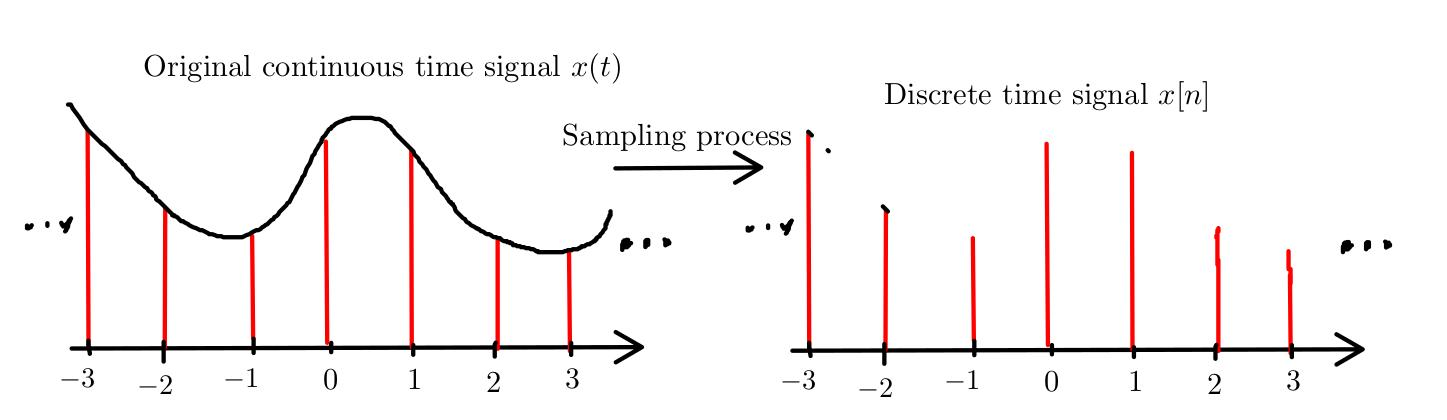
\includegraphics[width=0.6\textwidth]{discrete.jpg}
			\caption{Sampling process}			\label{fig:re1}
		\end{figure}
Như đã thảo luận ở \alert{Chương 1}, chúng ta có thể biểu diễn dữ liệu của chuỗi $x[n]$ như sau:
\begin{equation*}
	\begin{cases}
		\dots \\
		x[-2]=0.65\\
		x[-1]=0.4\\
		x[0]=0.9\\
		x[1]=0.96\\
		\dots \\
	\end{cases}
\end{equation*}
\end{frame}
\begin{frame}{Biểu diễn hệ thống LTI bằng đáp ứng xung}
	Cách biểu diễn chuỗi dữ liệu $x[n]$ như trên không tiện về mặt toán học do tương đối cồng kềnh và khó xử lý, chúng ta muốn tìm một cách biểu diễn $x[n]$ gọn hơn bằng \textbf{tổng vô hạn} như sau:

 \begin{figure}[h]
			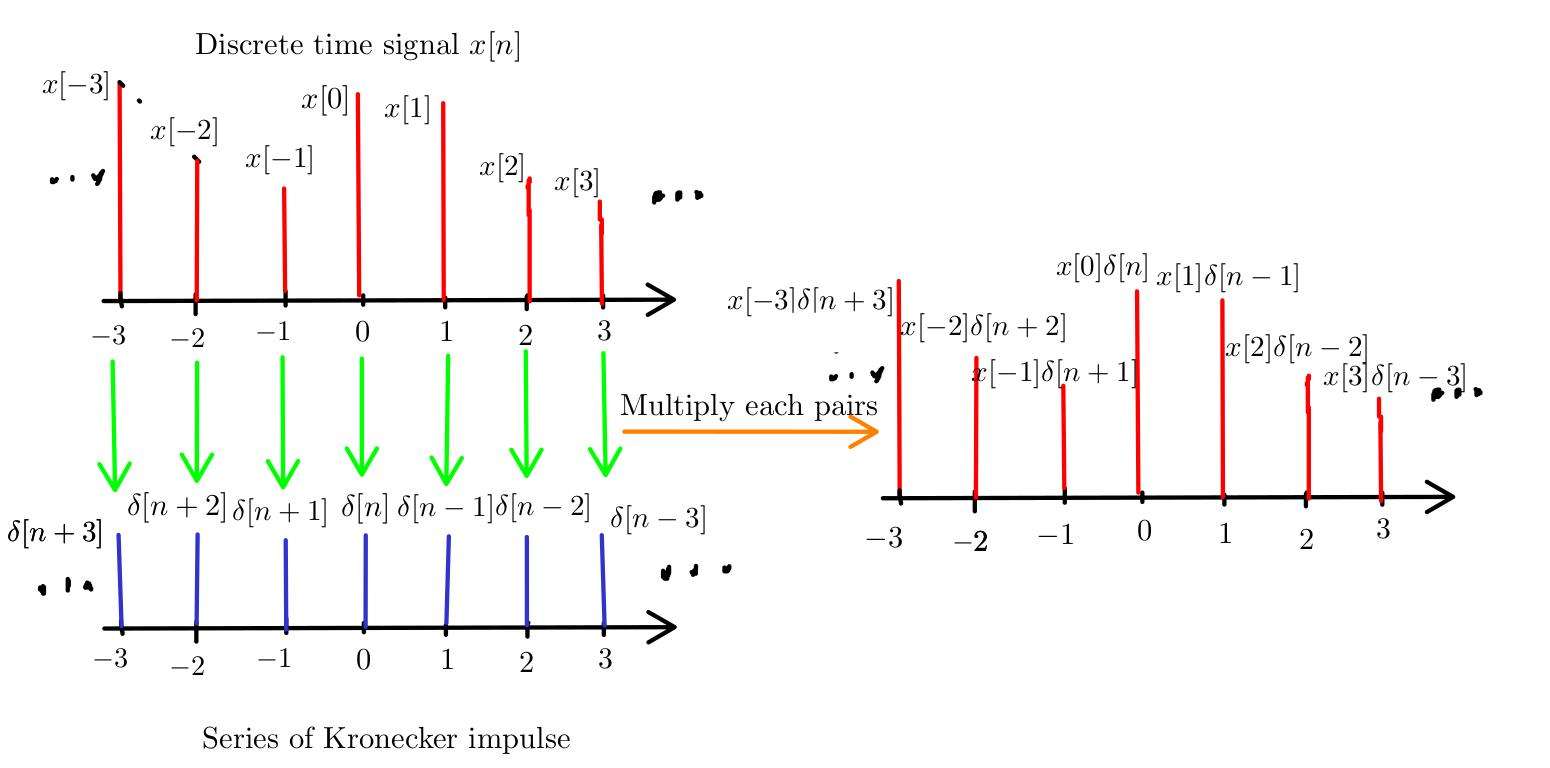
\includegraphics[width=1\textwidth]{process.jpg}
			\caption{Running sum visualization}\label{fig:re2}
		\end{figure}
\end{frame}
\begin{frame}{Biểu diễn hệ thống LTI bằng đáp ứng xung}
Từ hình minh họa trên, chúng ta thu được công thức biểu diễn $x[n]$ tổng quát bằng \textbf{tổng vô hạn} như sau:
\begin{block}{Công thức biểu diễn tín hiệu $x[n]$ tổng quát}
	$$x[n]=\sum_{k=-\infty}^{+\infty}x[k]\delta[n-k]$$
\end{block}
Suy ngẫm: tại sao tổng này còn được gọi là "running sum" ? Bạn hãy thử biểu diễn lại công thức trên và quan sát "cái gì" đang "chạy" ?
\\ Chúng ta tiếp tục cho tín hiệu đầu vào $x[n]$ trên đi qua một hệ thống LTI rời rạc có \alert{đáp ứng xung $h[n]$} (tạm thời bạn chưa cần hiểu khái niệm này, cứ công nhận trước đã), ta thu được tín hiệu ra $y[n]$ như sau:
\begin{figure}[h]
			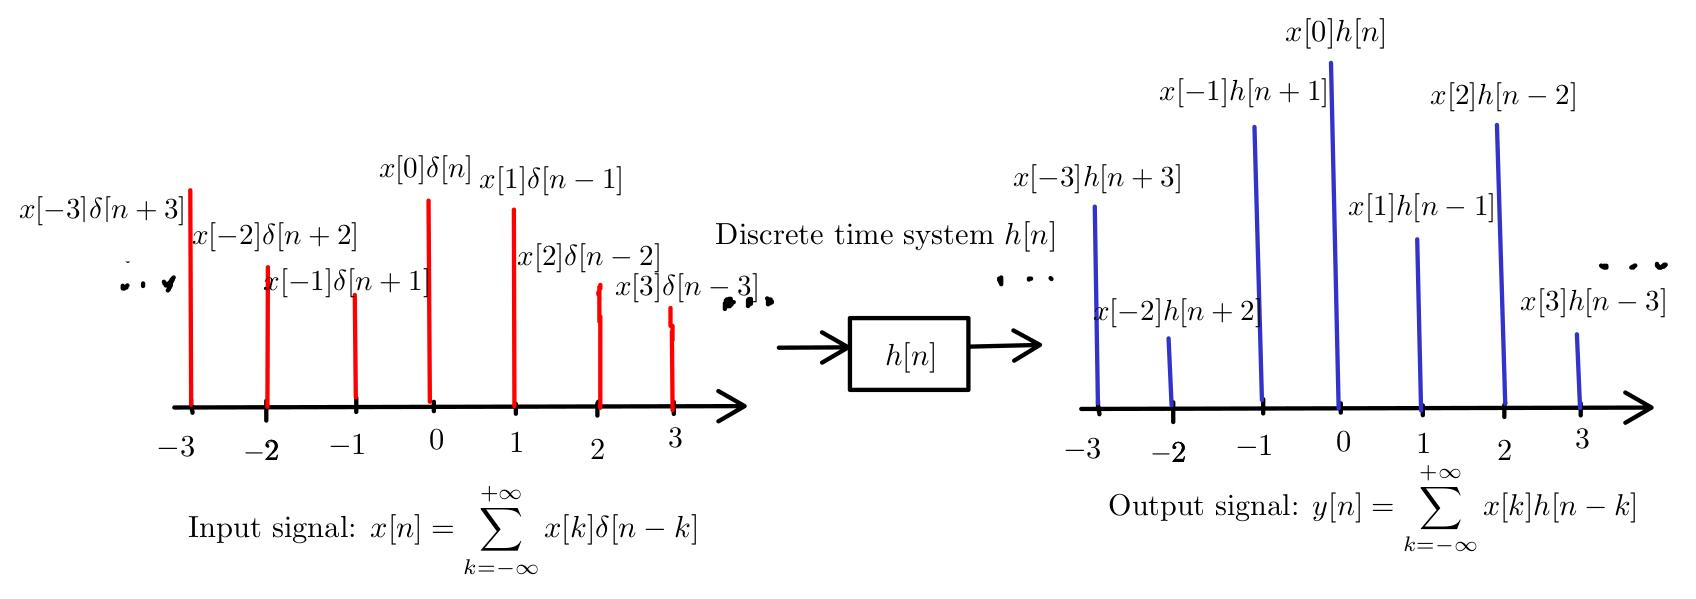
\includegraphics[width=0.8\textwidth]{system.jpg}
			\caption{In/output of LTI discrete time system}\label{fig:re3}
		\end{figure}
\end{frame}
\begin{frame}{Biểu diễn hệ thống LTI bằng đáp ứng xung}
	Quan sát tín hiệu ra $y[n]$, chúng ta nhận thấy hệ thống LTI rời rạc đã làm \textbf{biến đổi các thành phần $\delta[n-k]$ trong tín hiệu lối vào thành $h[n-k]$ ở tín hiệu lối ra}. Vậy ta có công thức biểu diễn tín hiệu $y[n]$ tổng quát (đầu ra của hệ thống LTI rời rạc) theo $x[n]$ (đầu vào của hệ thống LTI rời rạc) như sau:
	\begin{block}{Công thức biểu diễn tín hiệu $y[n]$ tổng quát}
		$$y[n]=\sum_{k=-\infty}^{+\infty}x[k]h[n-k]=\alert{x[n]*h[n]}$$
	\end{block}
	Toán tử $*$ được gọi là \alert{tích chập} (convolution). Vậy \alert{tích chập} là phép toán dùng để \textbf{tìm tín hiệu đầu ra $y[n]$ khi đã biết tín hiệu đầu vào $x[n]$ và đáp ứng xung của hệ thống LTI $h[n]$ }.
	\\ Suy ngẫm: xét tín hiệu đầu vào $x[n]=\delta[n]$ qua một hệ thống LTI $h[n]$. Tín hiệu ra $y[n]$ tức là đáp ứng của hệ thống với đầu vào là xung Kronecker (đáp ứng xung) có công thức như thế nào ? Bạn đã hiểu lý do tại sao $h[n]$ được gọi là \textbf{đáp ứng xung} của hệ thống chưa ?
	\\ Ví dụ: Cho một tín hiệu $x[n]=\alpha^{n}u[n]$ với $0<\alpha<1$ đi qua hệ thống LTI rời rạc có đáp ứng xung $h[n]=u[n]$, xác định tín hiệu ra của hệ thống.
\end{frame}
\begin{frame}{Biểu diễn hệ thống LTI bằng đáp ứng xung}

\begin{figure}[h]
			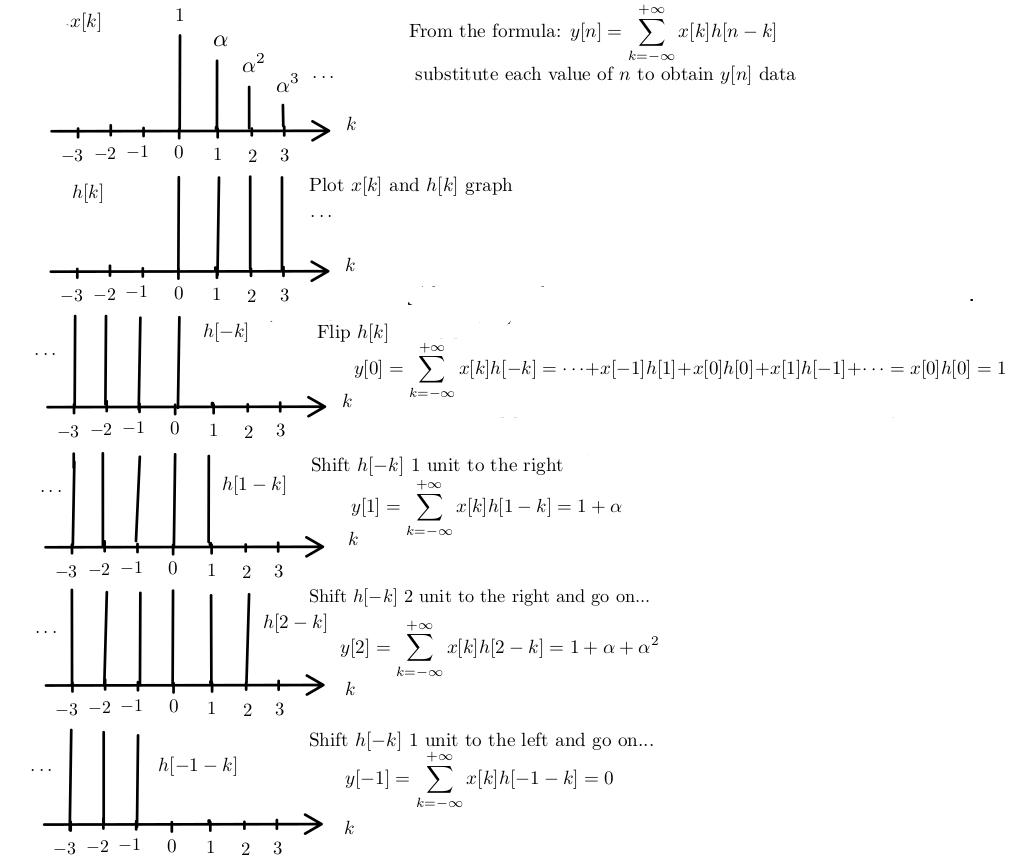
\includegraphics[width=0.8\textwidth]{conv.jpg}
			\caption{Perform convolution step by step}\label{fig:re4}
		\end{figure}
\end{frame}
\begin{frame}{Biểu diễn hệ thống LTI bằng đáp ứng xung}
Tổng quát hóa, nếu ta dịch $h[-k]$ đi $n$ đơn vị ($n$ không âm) thì:
$$y[n]=\sum_{k=-\infty}^{+\infty}x[k]h[n-k]=1+\alpha+\alpha^2+...+\alpha^n=\frac{1-\alpha^{n+1}}{1-\alpha}$$
Vậy ta thu được tín hiệu ra: $$y[n]=\frac{1-\alpha^{n+1}}{1-\alpha}u[n]=\frac{1}{1-\alpha}u[n]$$
Suy ngẫm: tại sao $h[1-k]$ lại là phiên bản \alert{dịch phải} của $h[-k]$ ? Giải thích câu trả lời của bạn.
\\ Đào sâu hơn một chút, từ công thức tính tích chập tổng quát:
$$y[n]=\sum_{k=-\infty}^{+\infty}x[k]h[n-k]=\alert{x[n]*h[n]}$$
Ta đặt $n-k=m$, dễ thấy:
$$y[n]=\sum_{m=+\infty}^{-\infty}x[n-m]h[m]=\sum_{m=-\infty}^{+\infty}x[n-m]h[m]=\alert{h[n]*x[n]}$$
Vậy ta kết luận \textbf{tích chập có tính giao hoán}.
\end{frame}
\begin{frame}{Biểu diễn hệ thống LTI bằng đáp ứng xung}
Suy ngẫm: hãy nghiệm lại tính chất giao hoán của tích chập qua bài toán tìm đầu ra của hệ thống LTI rời rạc có đáp ứng xung $h[n]=\alpha^n u[n]$ với $0<\alpha<1$ có đầu vào là xung đơn vị nhảy bậc $x[n]=u[n]$ (unit step response). Trong quá trình tính tích chập, bạn có để ý thấy "cái gì" đang "chạy" không ?
\subsubsection{Tính chất của tích chập rời rạc}
\begin{itemize}
	\item[-] Tính chất của tích chập rời rạc
\end{itemize}
\begin{block}{Tính chất của tích chập rời rạc}
	Giao hoán: $h_{1}[n]*h_{2}[n]=h_{2}[n]*h_{1}[n]$\\
	Phân phối: $h_{1}[n]*(h_{2}[n]+h_{3}[n])=h_{1}[n]*h_{2}[n]+h_{1}[n]*h_{3}[n]$\\
	Kết hợp: $(h_{1}[n]*h_{2}[n])*h_{3}[n]=h_{1}[n]*(h_{2}[n]*h_{3}[n])$
\end{block}
Suy ngẫm: các bạn hãy thử tự mình chứng minh lại $3$ tính chất trên. Gợi ý: đặt $h[n]=h_{2}[n]+h_{3}[n]$ làm ẩn phụ. Tính chất kết hợp tương đối khó chứng minh, nhưng có thể thử theo hướng sau (optional):
\begin{equation*}
	\begin{split}
		(h_{1}[n]*h_{2}[n])*h_{3}[n]&=\sum_{m=-\infty}^{+\infty}\left(\sum_{k=-\infty}^{+\infty}h_{1}[k]h_{2}[m-k]\right)h_{3}[n-m]\\
					    &=\sum_{k=-\infty}^{+\infty}\left(\sum_{m=-\infty}^{+\infty}h_{2}[m-k]h_{3}[n-m]\right)h_{1}[k]\\
					    &=h_{1}[n]*(h_{2}[n]*h_{3}[n])\\
	\end{split}
\end{equation*}
\end{frame}
\begin{frame}{Biểu diễn hệ thống LTI bằng đáp ứng xung}
\begin{itemize}
	\item[-] Khảo sát tính chất hệ thống LTI rời rạc
\end{itemize}
\subsubsection{Khảo sát tính chất của hệ thống LTI rời rạc}
 Do các hệ thống LTI rời rạc đã có sẵn tính chất \textbf{tuyến tính} và \textbf{bất biến}, nên ta chỉ cần khảo sát $3$ tính chất còn lại gồm: \alert{không nhớ}, \alert{nhân quả} và \alert{ổn định}. Một hệ thống LTI bất kỳ có thể được biểu diễn qua phép tính tích chập như sau:
 \begin{equation*}
	 \begin{split}
		 y[n]&=x[n]*h[n]=\sum_{k=-\infty}^{+\infty}x[k]h[n-k]=\sum_{k=-\infty}^{+\infty}x[n-k]h[k] \text{     (commutative property)}\\
		     &=\dots+x[n-2]h[2]+x[n-1]h[1]+x[n]h[0]+x[n+1]h[-1]+x[n+2]h[-2]+\dots \\
	\end{split}
\end{equation*}
Quan sát đầu vào-ra của hệ thống, rất hiển nhiên ta có thể nhận ra ngay để hệ thống này \alert{không nhớ} thì tất cả các hạng tử khác $x[n]h[0]$ phải bằng $0$ (các bạn có thể xem lại lý thuyết phần \alert{Hệ thống} của \alert{Chương 1} nếu cần). Vậy ta suy ra $h[n]=0 \;(\forall n\neq 0 )$
\\ Tương tự, để hệ thống này \alert{nhân quả} thì tất cả các hạng tử lớn hơn $n$ (tương lai của thời điểm $n$) như $x[n+1]h[-1],x[n+2]h[-2],\dots$ phải bằng $0$. Vậy ta suy ra $h[n]=0\;(\forall n<0)$.
\\ Để hệ thống này \alert{ổn định}, ta tạo ràng buộc $|x[n]|<B$, lúc này ta có:
\begin{equation*}
\begin{split}
	|y[n]|=|x[n]*h[n]|=\left|\sum_{k=-\infty}^{+\infty}x[k]h[n-k]\right|<\sum_{k=-\infty}^{+\infty}\left|x[k]h[n-k]\right|&<B\sum_{k=-\infty}^{+\infty}|h[n-k]| \\
	      &= B\sum_{n=-\infty}^{+\infty}|h[n]|\\
\end{split}
\end{equation*}
\end{frame}
\begin{frame}{Biểu diễn hệ thống LTI bằng đáp ứng xung}
	Vậy để hệ thống \alert{ổn định}, ta suy ra: $$\sum_{n=-\infty}^{+\infty}|h[n]|<+\infty$$
	\begin{block}{Tính chất hệ thống LTI rời rạc}
Không nhớ: $h[n]=0\;(\forall n \neq 0)$\\
Nhân quả: $h[n]=0\;(\forall n<0)$\\
Ổn định: 
$$\sum_{n=-\infty}^{+\infty}|h[n]|<+\infty$$
\end{block}
Suy ngẫm: hệ thống LTI rời rạc có đáp ứng xung $h[n]=u[n]$ có những tính chất nào ? Nếu hệ thống này \textbf{không ổn định}, bạn hãy tìm một ví dụ để chứng minh điều đó.
\end{frame}
\begin{frame}{Biểu diễn hệ thống LTI bằng đáp ứng xung}
\subsection{Hệ thống LTI liên tục}
\begin{itemize}
	\item Hệ thống LTI liên tục
\end{itemize}
\subsubsection{Tích chập liên tục}
\begin{itemize}
	\item[-] Tích chập liên tục
\end{itemize}
Phần chứng minh công thức tích chập liên tục tương đối khó nên các bạn có thể bỏ qua (optional) và xem thẳng đến slide công thức.

\begin{figure}[h]
			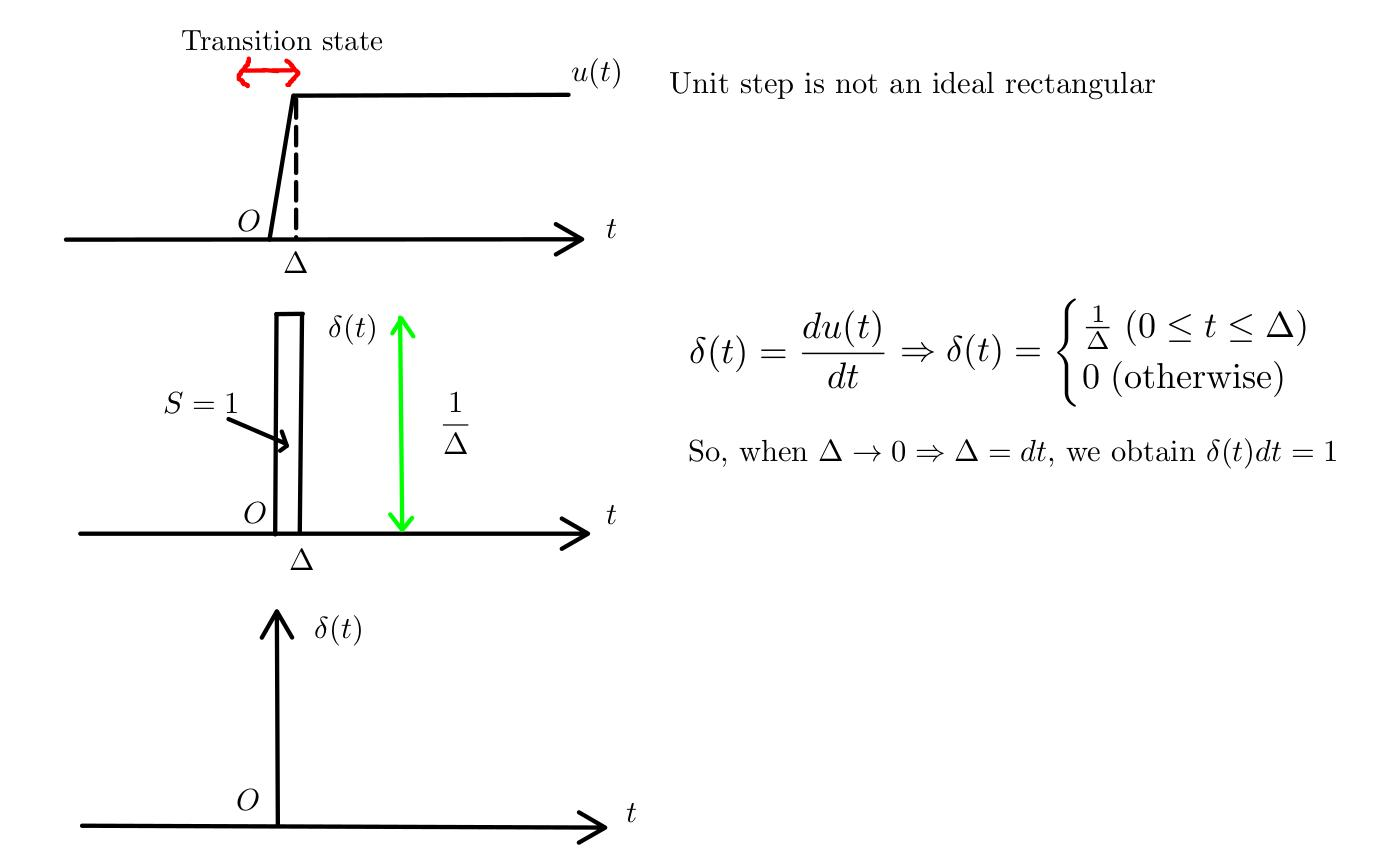
\includegraphics[width=0.9\textwidth]{dirac.jpg}
			\caption{Go deeper into Dirac impulse}\label{fig:re5}
		\end{figure}
\end{frame}
\begin{frame}{Biểu diễn hệ thống LTI bằng đáp ứng xung}
\begin{figure}[h]
			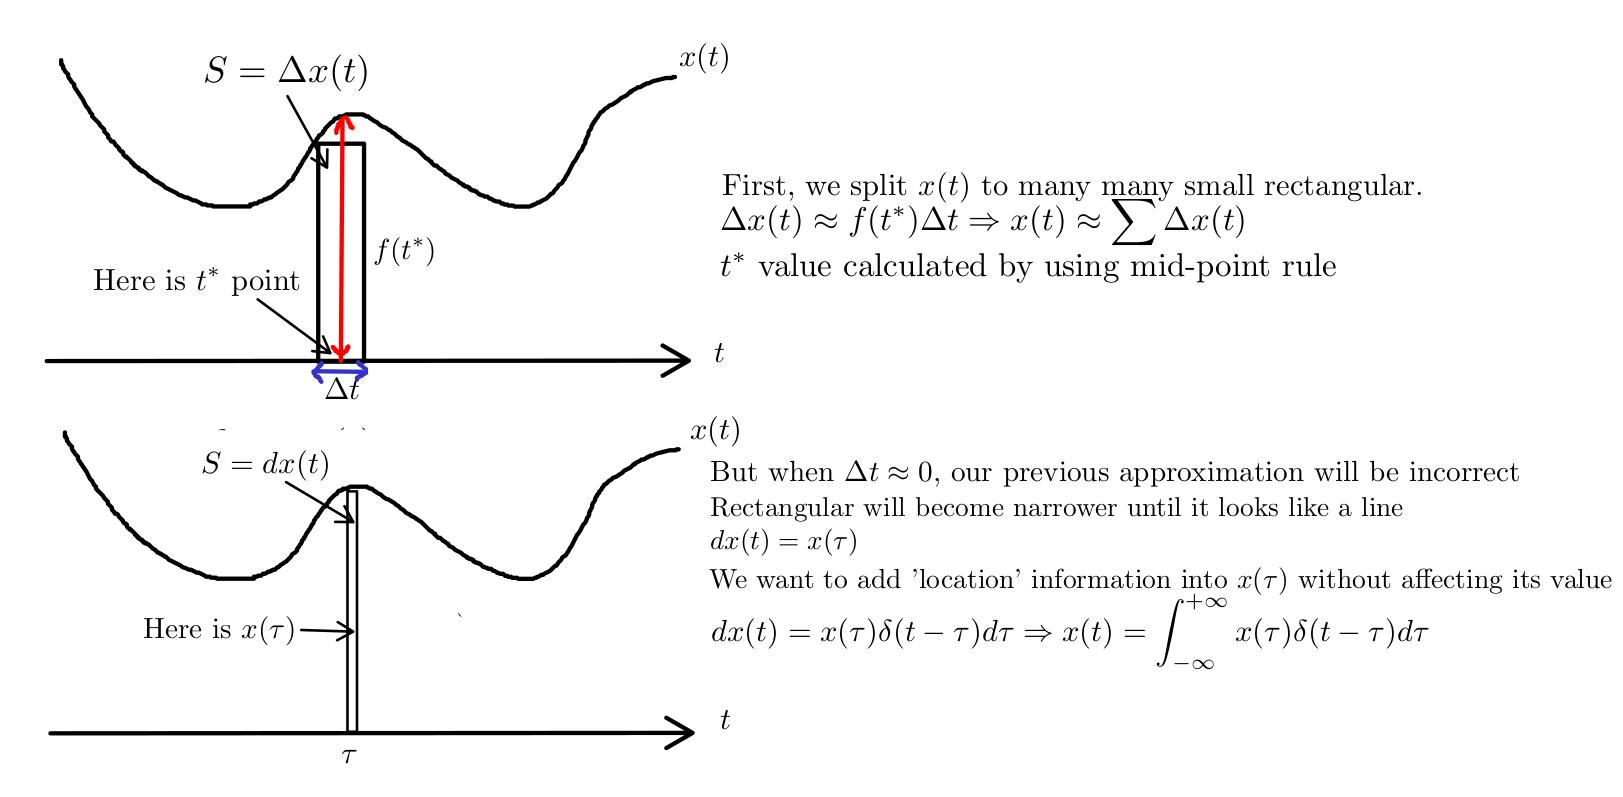
\includegraphics[width=1\textwidth]{tau.jpg}
			\caption{Represent $x(t)$ in integral form}\label{fig:re6}
		\end{figure}
\end{frame}
\begin{frame}{Biểu diễn hệ thống LTI bằng đáp ứng xung}
Tương tự như hệ thống LTI rời rạc đã trình bày ở trên, khi ta cho tín hiệu đầu vào $x(t)$ đi qua hệ thống LTI liên tục có đáp ứng xung $h(t)$, ta thu được tín hiệu đầu ra $y(t)$ có công thức như sau:
\begin{block}{Công thức biểu diễn tín hiệu $x(t)$ và $y(t)$ tổng quát}
	\begin{equation*}
	\begin{split}
		x(t)&=\int_{-\infty}^{+\infty}x(\tau)\delta(t-\tau)d\tau\\
		y(t)&=\int_{-\infty}^{+\infty}x(\tau)h(t-\tau)d\tau=\alert{x(t)*h(t)}\\
	\end{split}
	\end{equation*}
\end{block}
\end{frame}
\end{document}

